\documentclass[10pt,twocolumn,letterpaper]{article}
\usepackage[review]{cvpr}
%% This file contains a number of tweaks that are typically applied to the main document.
%% They are not enabled by default, but can be enabled by uncommenting the relevant lines.


%%
%% Official support for 2-column teaser figure
%%
\usepackage{cuted} %< for strip environment

%%
%% For auto-referencing of figures (see fig/teaser.tex and \label{} therein) 
%%
\usepackage{currfile} %< for \currfilebase macro

%%
%% caption and (global) spacing overrides
%%
\usepackage{caption} %< for "\captionof" commands (teaser)
% \setlength{\abovecaptionskip}{.5em} % space above caption
% \setlength{\belowcaptionskip}{1em} % space below caption

%%
%% Inline annotations; for predefined colors, refer to "dvipsnames" in the xcolor package:
%% https://tinyurl.com/overleaf-colors
%%
\newcommand{\red}[1]{{\color{red}#1}}
\newcommand{\todo}[1]{{\color{red}#1}}
\newcommand{\TODO}[1]{\textbf{\color{red}[TODO: #1]}}
%%
%% Disable for camera ready / submission by uncommenting these lines:
%%
% \renewcommand{\TODO}[1]{}
% \renewcommand{\todo}[1]{#1}

%%
%% Work harder in optimizing text layout. Typically shrinks text by 1/6 of page, enable
%% it at the very end of the writing process, when you are just above the page limit.
%%
% \usepackage{microtype}

%%
%% Fine-tune paragraph spacing.
%%
% \renewcommand{\paragraph}[1]{\vspace{.5em}\noindent\textbf{#1.}}

%%
%% Globally adjusts space between figure and caption.
%%
% \setlength{\abovecaptionskip}{.5em}

%%
%% Allows "the use of \paper to refer to the project name"
%% with automatic management of space at the end of the word.
%%
% \usepackage{xspace}
% \newcommand{\paper}{ProjectName\xspace}

%%
%% Commonly used math definitions.
%%
% \DeclareMathOperator*{\argmin}{arg\,min}
% \DeclareMathOperator*{\argmax}{arg\,max}

%%
%% Tighten underline.
%%
% \usepackage{soul}
% \setuldepth{foobar}

%%
%% Reconfigure paragraph (tweaks spacing)
%%

\usepackage{booktabs}
\usepackage{adjustbox}
\usepackage{multirow}
\usepackage{amsmath,amssymb}
\usepackage{graphicx}
\usepackage{xspace}
\usepackage{tikz}
\usetikzlibrary{positioning,fit,calc}
\newcommand{\ours}{LineageRAFT\xspace}
\newcommand{\rodsim}{\textsc{RodSim}\xspace}
\definecolor{cvprblue}{rgb}{0.21,0.49,0.74}
\usepackage[pagebackref,breaklinks,colorlinks,allcolors=cvprblue]{hyperref}

\def\paperID{*****}
\def\confName{CVPR}
\def\confYear{2027}

\title{Lineage from Two Snapshots, Learned without Lineage Labels}

\author{Anonymous CVPR submission}

\begin{document}
\maketitle
\begin{strip}
\centering
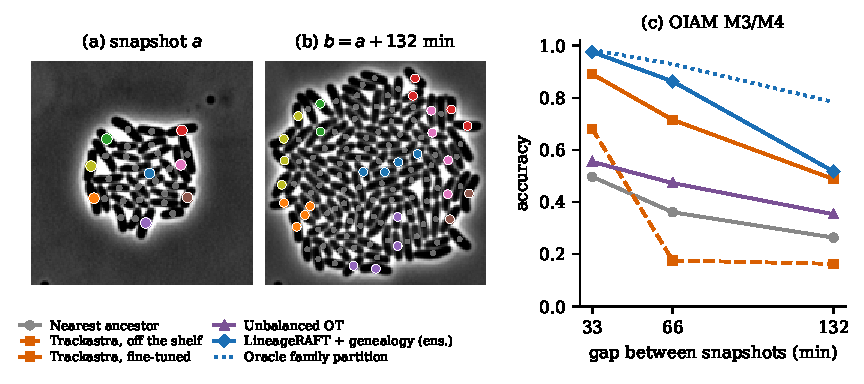
\includegraphics[width=\linewidth]{fig/teaser.pdf}
\captionsetup{hypcap=false}
\captionof{figure}{\textbf{Two-snapshot ancestry.} (a) A \emph{C.~glutamicum} microcolony and (b) the same colony 132 minutes later; eight ancestors in (a) and their descendants in (b) are coloured, all other cells are grey. Descendant families are displaced and interleaved by growth. (c) Accuracy on One-in-a-Million (OIAM) movies M3/M4 (rows of \cref{tab:oiam}; \ours: three-seed ensemble with genealogy decoder). A recent learned tracker given ground-truth masks falls below nearest assignment from 66 minutes on unless fine-tuned at each gap on annotated lineage; unbalanced optimal transport gains little. Family registration with single-snapshot genealogy stays above all of them and approaches an oracle that knows the family partition at short gaps.}
\captionsetup{hypcap=true}
\label{fig:teaser}
\end{strip}

\begin{abstract}
Time-lapse microscopy reconstructs cell lineages by linking cells frame to frame, which requires dense imaging that is phototoxic, storage-hungry and often impossible.
We ask how much lineage survives sparse imaging: given two snapshots of a growing bacterial colony taken $H$ minutes apart, assign every cell in the later one to its ancestor in the earlier one.
Between snapshots cells divide several times and colonies deform, so trackers, optimal transport and point-set registration degrade sharply.
We propose \ours, which registers descendant \emph{families} rather than cells: it iteratively moves one predicted family centre per ancestor and scores candidates relative to it.
On One-in-a-Million movies its window-averaged accuracy is 0.96 at a 33-minute gap and 0.47 at 132 minutes, where an ancestor has up to eight descendants; composing its links over 13 of 133 frames recovers two hours of lineage for 0.99 of cells, where off-the-shelf Trackastra, even given true masks, needs 34 frames.
Two routes avoid lineage annotation.
Trained only on a colony simulator, \ours beats every positions-only baseline, optimal transport and forward simulation included, zero-shot on all 27 sequences of four bacterial datasets and, in a pre-registered blind test, on all 28 colonies of three unseen subsets; a plain learned matcher trained the same way does as well, so this transfer is the simulator's.
Chaining one-frame links under a binary-fission prior through unannotated time-lapses yields pseudo-lineage that trains \ours to within 0.02--0.05 of annotation.
Decoded with a single-image genealogy network, this annotation-free pipeline beats a transformer tracker fine-tuned on annotated lineage and decoded the same way by 0.02--0.03 at 33 and 66 minutes (0.07--0.11 against its own output) and matches it at 132.
We also report pre-registered failures: fields of many tiny colonies and steady-state chambers.
\end{abstract}

\section{Introduction}
\label{sec:intro}

Who descends from whom is the central question of developmental biology, microbiology and cancer research.
Imaging answers it by tracking: segment cells in every frame of a time-lapse movie and link them across consecutive frames~\cite{ulman2017objective,maska2023ctc}.
Linking is easy only when frames are dense relative to cell motion and division.
Dense imaging, however, costs light dose, storage and instrument time, and many experiments cannot provide it at all: long experiments limited by phototoxicity, high-throughput screens that revisit each field only occasionally, or archives in which most frames were never kept.

We ask how much lineage can be recovered from the sparsest possible record: \emph{two snapshots} of the same population separated by $H$ minutes.
At $H{=}33$ minutes in a dense bacterial colony roughly every second cell has divided; at $H{=}132$ minutes each ancestor has up to eight descendants that have been pushed away by the growth of hundreds of neighbours (\cref{fig:teaser}).
The task is neither tracking (there is no smooth trajectory to follow) nor registration (the two point sets differ in size and topology).
We show that it is nonetheless learnable, and that it never needs annotated lineage: the learning signal can come from simulation, or from unannotated time-lapses labelled under a binary-fission constraint.

\paragraph{Family registration.}
A descendant family moves as a unit: its members are siblings and cousins packed together, displaced by the same pressure field.
\ours therefore predicts, for every ancestor, the centre of its descendant family at time $b$ and refines that centre through $T$ rounds of local cross-attention, in the spirit of iterative flow refinement~\cite{teed2020raft}.
Targets are scored against candidate ancestors by their offset from the refined centres; freezing the centres in an otherwise identical network costs 0.10 accuracy at 33 and 66 minutes.
A single network is trained across horizons from 8 to 240 minutes.

\paragraph{Learning lineage without lineage labels.}
Lineage annotations are scarce, and a model trained on one experiment transfers poorly to others (\cref{tab:external}).
A model trained only on \rodsim, an agent-based simulator of growing rod-shaped colonies, transfers well: it beats ten positions-only geometric, optimal-transport, registration and simulation baselines on all 27 bacterial sequences of four real datasets it was never trained on, by 3 to 10 points of accuracy over the best of them (three-seed mean); a plain learned matcher trained on the same simulations does as well, so the transfer is the simulator's.
A pre-registered blind test (protocol and hypotheses fixed in a file before the data were downloaded) confirms this on 28 unseen colonies grown in another medium, against the same baselines; earlier blind tests delimit its scope: it assumes a contiguous population expanding by its own growth, and fails on fields of many separate microcolonies and on steady-state chambers.
The remedy comes from biology.
Between consecutive frames, binary fission reduces lineage to an assignment in which each cell either persists or is replaced by daughters on either side of its centre along its axis; chaining such links through a dense \emph{unannotated} time-lapse yields pseudo-lineage at horizons up to four hours, 0.88--0.98 correct on the One-in-a-Million (OIAM) movies.
Trained on pseudo-lineage of three unannotated OIAM movies, \ours comes within 0.02--0.05 of the annotated model over all windows; decoded, it beats Trackastra~\cite{gallusser2024trackastra} fine-tuned on annotated lineage at 33 and 66 minutes and matches it at 132.
Bootstrapped self-labelling from the other half of a dataset's movies, fixed in advance, improves the simulation-trained model on all seven sources of our blind tests (pre-registered on the last three; on the four earlier ones, simpler Hungarian links did even better).
One dense, unannotated movie per organism could thus replace dense imaging later.

\paragraph{Genealogy in a single image.}
An oracle analysis shows that, given the true partition of targets into families, assignment accuracy at $H{=}132$ rises from 0.52 (our best model) to 0.78: errors pick a neighbour of the true ancestor, so the bottleneck is grouping, not coarse motion.
Grouping is visible in one frame: a network that predicts the time since two neighbours' lineages split, from a single phase-contrast image, detects same-family pairs with 0.97/0.91/0.70 average precision at $H{=}33/66/132$.
Coupling these affinities with \ours in a Potts mean-field decoder improves every base model at every gap.
The same network can be trained on \rodsim alone once the simulator randomises how cells divide, giving a pipeline with no real lineage label, though it then relies mostly on geometry.

\paragraph{Contributions.}
(1)~We formalise \emph{two-snapshot ancestry} and assemble a benchmark spanning six bacterial and human-cell datasets and three horizons, with cell-level accuracy and family-level biological readouts.
(2)~We propose \ours, an iterative family-registration network that resolves crowded colonies, where a learned matcher of the same capacity trails it by 0.10.
(3)~We show that \ours needs no annotated lineage: simulated colonies, or fission-constrained pseudo-lineage from unannotated time-lapses, suffice, including in pre-registered blind tests.
(4)~We predict genealogy from a single image and use it in a partition-aware decoder.

\section{Related work}
\label{sec:related}

\paragraph{Cell tracking.}
Classical pipelines, including bacterial ones~\cite{stylianidou2016supersegger,lugagne2020delta,ollion2019bacmman,ollion2024distnet2d}, link segmented cells between consecutive frames by nearest neighbour or linear assignment~\cite{jaqaman2008robust,ershov2022trackmate}, optionally with global optimisation over a tracking graph~\cite{bragantini2024ultrack}.
Learned trackers predict associations with graph networks or transformers~\cite{ben2022graph,gallusser2024trackastra,joy2021hipsc,fedorchuk2025deepkymo}, and the Cell Tracking Challenge~\cite{ulman2017objective,maska2023ctc} benchmarks them on dense movies.
Whole-embryo systems combine learned detectors with integer linear programs~\cite{malinmayor2023linajea,hirsch2022celegans,sugawara2022elephant}; Tui~\cite{chang2026tui} adds expert correction across generations.
All assume that consecutive frames overlap substantially in appearance and position; with two snapshots the tracking graph has a single layer, so global optimisation reduces to one constrained assignment, the setting of our optimal-transport baselines.
The One-in-a-Million dataset~\cite{seiffarth2024oiam} reports that tracking quality falls with frame interval and population size; we study a single long interval.

\paragraph{Correspondence and flow.}
\ours borrows iterative refinement from optical flow~\cite{teed2020raft}, attention-based matching with a dustbin from feature matching~\cite{sarlin2020superglue,lindenberger2023lightglue}, and, closest in mechanism, the per-query reference point that DETR-style detectors refine by attending around it~\cite{carion2020detr,zhu2021deformable,liu2022dabdetr}, akin to voting for object centres~\cite{qi2019votenet}.
Here a query is an ancestor and its reference point the centre of a set of points that did not exist at $a$.
Scene flow~\cite{liu2019flownet3d,wu2020pointpwc,puy2020flot}, point-cloud registration~\cite{wang2019dcp,yew2020rpmnet} and point tracking~\cite{karaev2024cotracker} follow the same objects; here the mapping is one-to-many.

\paragraph{Learning without labels.}
Randomised synthetic data~\cite{tobin2017domain} trains flow~\cite{dosovitskiy2015flownet} and robot policies; an agent-based colony model~\cite{rudge2012cellmodeller} gives us unlimited lineage-annotated pairs.
Correspondence can be learned from unlabelled video through cycle consistency or random walks over short time steps~\cite{wang2019learning,jabri2020space}.
Our self-labels likewise come from where the problem is easy, one frame, and supervise where it is hard, hours; but they are produced by a biological constraint, binary fission, rather than by the model itself.

\paragraph{Lineage from static data.}
Genetic lineage tracing recovers trees from barcodes in a single sample~\cite{wagner2020lineage}.
Between unpaired snapshots of single-cell profiles, unbalanced optimal transport with a growth term infers ancestor--descendant couplings~\cite{schiebinger2019optimal}, also with lineage barcodes~\cite{forrow2021lineageot} or spatial coordinates~\cite{klein2025moscot}; we evaluate it, and non-rigid point-set registration~\cite{myronenko2010cpd}, as baselines in physical space.
Lineage trees can also be inferred from phenotypic similarity of single cells~\cite{kuang2025celltreeqm}; we show that image appearance alone carries a coarse genealogical signal: recent sisters, and less so cousins, can be identified in one frame.

\section{Two-snapshot ancestry}
\label{sec:problem}

\paragraph{Task.}
We observe a population at times $a$ and $b{=}a{+}H$.
Each snapshot provides cell detections $\mathcal{A}{=}\{\mathbf{x}_i\}_{i=1}^{N_a}$ and $\mathcal{B}{=}\{\mathbf{y}_j\}_{j=1}^{N_b}$ (centroid, and optionally major/minor axis and orientation) and, when available, the image.
For every target $j$ we predict its ancestor $\pi(j)\in\mathcal{A}\cup\{\varnothing\}$, the cell at time $a$ whose lineage contains $j$; $\varnothing$ denotes cells that entered the field of view.
No intermediate frame and no identity information is available at inference.
Ground-truth ancestry comes from full-resolution tracking and is used only for training and evaluation.

\paragraph{Metrics.}
Accuracy is the fraction of evaluable targets (inside the field of interest, with a visible ancestor) assigned to the correct ancestor, averaged over windows (one snapshot pair of one movie); weighting by cells instead counts dense windows more and gives lower numbers (Supp.~E).
At the family level we compare biological readouts of the predicted and true families (size control; family-size spread in Supp.~H).
We report results separately on \emph{dense} windows ($N_a{>}200$), where ambiguity is highest.

\paragraph{Data.}
\cref{tab:datasets} summarises the datasets.
\emph{OIAM}~\cite{seiffarth2024oiam}: five \emph{C.~glutamicum} microcolony movies (M0--M4) with over 1.4M annotated instances; we train in-domain models on M0--M2 (or four movies in leave-one-movie-out) and evaluate at $H\in\{33,66,132\}$ minutes.
\emph{FAST}~\cite{meacock2023fast}: seven \emph{E.~coli} microcolonies with manually corrected lineages.
\emph{recA} and \emph{rpsM}: nine \emph{E.~coli} microcolonies each from the raw data of~\cite{vanvliet2018spatially} (also FAST's source), with other reporters, dates and colonies and uncurated Schnitzcells lineages (audited in Supp.~E).
\emph{LFCT}~\cite{gachloo2026lfct}: one field of motile MDA-MB-231 breast cancer cells; \emph{T98G}~\cite{chang2026tui}: one field of T98G glioblastoma cells under electrotaxis.
The last two are sparse and motile, a regime deliberately unlike the simulator.
External datasets are never used for training.
The window lists, the \rodsim simulator, code and trained models will be released.

\begin{table}[t]
\centering\small
\setlength{\tabcolsep}{3pt}
\resizebox{\linewidth}{!}{%
\begin{tabular}{lllrrr}
\toprule
Dataset & Organism & Gaps (min) & Seq. & Windows & max $N_a$ \\
\midrule
OIAM (M3/M4) & \emph{C. glutamicum} & 33/66/132 & 2 & 109 & 1359 \\
FAST & \emph{E. coli} & 35/65/130 & 7 & 1409 & 124 \\
recA & \emph{E. coli} & 30/60/120 & 9 & 345 & 108 \\
rpsM & \emph{E. coli} & 30/60/120 & 9 & 900 & 113 \\
LFCT & MDA-MB-231 & 30/60/120 & 1 & 1141 & 13 \\
T98G & T98G & 30/70/130 & 1 & 88 & 74 \\
\bottomrule
\end{tabular}}
\caption{\textbf{Evaluation datasets.} Windows pool all gaps.}
\label{tab:datasets}
\end{table}

\section{Method}
\begin{figure*}[t]
\centering
\resizebox{\linewidth}{!}{%
\begin{tikzpicture}[
  font=\scriptsize, >=stealth, node distance=4mm,
  box/.style={draw, rounded corners=2pt, align=center, minimum height=7mm, inner sep=2pt, fill=white},
  data/.style={box, fill=gray!10},
  net/.style={box, fill=blue!8},
  sim/.style={box, fill=orange!12},
  loop/.style={draw, dashed, rounded corners=4pt, inner sep=3pt, blue!50!black}]
% inputs, each tokenised in its canonical frame and encoded with local attention
\node[data, text width=24mm] (A) {snapshot $a$:\\$\{\mathbf{x}_i\}_{i\le N_a}$, tokens + local attention};
\node[data, text width=24mm, below=5mm of A] (B) {snapshot $b{=}a{+}H$:\\$\{\mathbf{y}_j\}_{j\le N_b}$, tokens + local attention};
\node[data, text width=24mm, below=4mm of B] (I) {image at $b$};
% loop: X1 -> U -> X2 -> X1
\node[net, right=15mm of A] (X1) {(i, ii) ancestors attend\\to targets near $\mathbf{c}_i^{(t-1)}$};
\node[net, right=4mm of X1] (U) {(iii) $\mathbf{c}_i^{(t)}{=}\mathbf{c}_i^{(t-1)}{+}\Delta_t$};
\node[net, below=5mm of X1] (X2) {(iv) targets attend\\to nearest centres};
\node[loop, fit=(X1)(U)(X2), label={[blue!50!black, font=\scriptsize]below right:{family registration, $t{=}1..T$}}] (L) {};
\node[net, right=6mm of U] (S) {scores $p_{ji}$\\+ dustbin};
\node[net, right=4mm of S] (P) {Potts mean\\field (Eq.~1)};
\node[box, right=4mm of P] (O) {ancestor\\$\pi(j)$};
% genealogy
\node[net, right=6mm of I] (G) {pair CNN: $P(\tau_{jk}{<}H)$};
% real-data inset: centres moving through the rounds
\node[anchor=north west, inner sep=0] (IN) at ([xshift=4mm, yshift=-3mm]O.north east) {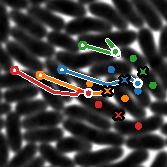
\includegraphics[height=29mm]{fig/centre_inset.pdf}};
\node[anchor=south, font=\scriptsize] at (IN.north) {real data, $H{=}66$ min};
\draw[->] (A) -- node[above, font=\scriptsize] {$\mathbf{c}^{(0)}_i$} node[below, font=\tiny] {radial/Darcy} (X1);
\draw[->] (I) -- (G);
\draw[->] (X1) -- (U);
\draw[->] (U.south) |- (X2.east); \draw[->] (X2.north) -- (X1.south);
\draw[->] (B) -- (X2);
\draw[->] (U) -- (S); \draw[->] (S) -- (P); \draw[->] (G) -| (P); \draw[->] (P) -- (O);
\end{tikzpicture}}
\caption{\textbf{Overview.} For every ancestor \ours keeps one estimate of its descendant-family centre and refines it over $T$ rounds of cross-attention to nearby targets; targets then score candidate ancestors by their offset from the refined centres. A genealogy network predicts from the target image whether neighbouring cells share an ancestor $H$ minutes ago, and a Potts mean-field decoder combines both. The same network is trained on \rodsim colonies, self-labelled time-lapses or annotated lineage. Right: in a dense OIAM window, centres move from initialisation (open) to $\mathbf{c}_i^{(T)}$ (filled) towards the true centroids (crosses) of the descendants (dots).}
\label{fig:method}
\end{figure*}

\label{sec:method}

\subsection{\ours: iterative family registration}
\label{sec:raft}

\paragraph{Tokens.}
\cref{fig:method} gives an overview. Each cell becomes a token built only from quantities available in its own snapshot, plus four scalars shared by the window: $\log_2 H$, $\log(N_b/N_a)$, $\log N_a$ and $\log N_b$.
Positions are expressed in a canonical frame: centred on the snapshot centroid and divided by the median nearest-neighbour spacing $s$; ancestor positions are additionally scaled by $\sqrt{N_b/N_a}$, the isotropic expansion that keeps the population density constant.
Per-cell features add orientation as $(\cos 2\theta,\sin 2\theta)$, log major and minor axes (when shapes are used), and the vector to the nearest image border, through which cells leave.

\paragraph{Encoder.}
Two layers of local attention operate within each snapshot: every token attends to its $k{=}12$ nearest neighbours, with keys and values augmented by an MLP embedding of the relative offset.
A global context token, pooled over the snapshot, is broadcast back.

\paragraph{Iterative family registration.}
Let $\mathbf{c}_i^{(0)}$ be an initial estimate of the centre of ancestor $i$'s descendant family at time $b$ (the scaled position above, or the advection of $\mathbf{x}_i$ through a Darcy growth-pressure field, \cref{sec:darcy}).
For $t=1,\dots,T$ ($T{=}4$):
(i) ancestor $i$ cross-attends to the $24$ targets nearest $\mathbf{c}_i^{(t-1)}$, with relative offsets $\mathbf{y}_j-\mathbf{c}_i^{(t-1)}$ as positional keys;
(ii) ancestors exchange information with their spatial neighbours;
(iii) the centre is updated, $\mathbf{c}_i^{(t)}=\mathbf{c}_i^{(t-1)}+\Delta_t(\mathbf{h}_i)$, with a zero-initialised head;
(iv) targets attend to their nearest centres, so a target's representation knows which families compete for it.
Updating a single point per family, rather than a dense field, matches the structure of the problem: families move rigidly to first order while the population as a whole deforms non-uniformly.

\paragraph{Assignment.}
Each target $j$ is scored against the $k_{\text{out}}{=}24$ ancestors whose final centres are closest, by an MLP over $[\mathbf{h}_j,\mathbf{h}_i,(\mathbf{y}_j-\mathbf{c}_i^{(T)})/4,\|\mathbf{y}_j-\mathbf{c}_i^{(T)}\|/4]$, plus a learned dustbin logit for targets without a visible ancestor~\cite{sarlin2020superglue}.

\paragraph{Training.}
Windows are sampled from every pair of frames with $H$ log-uniform in $[8,240]$ minutes.
The loss combines cross-entropy over candidates and dustbin, a deeply supervised centre loss $\sum_t 0.8^{T-t}\min(\|\mathbf{c}_i^{(t)}-\bar{\mathbf{y}}_{\mathcal{F}(i)}\|,10)$ towards the true family centroid $\bar{\mathbf{y}}_{\mathcal{F}(i)}$ (the mean position of $i$'s descendants), a binary same-family loss on target pairs, and an optional consistency term that asks the assignment overlap $\sum_i p_{ji}p_{ki}$ to agree with family membership.
Models trained on \rodsim or for transfer are augmented with random rotations and reflections of the canonical frame; in-domain OIAM models are trained without them, since the growth chambers fix a preferred axis.

\subsection{\rodsim: randomised colony simulation}
\label{sec:sim}

\rodsim grows colonies of rod-shaped cells from one to four founders until 900--2{,}200 cells.
Each cell is a chain of spheres of radius $0.5\,\mu$m; overlapping cells repel through soft contacts with anisotropic drag and torque, and elongate exponentially at a rate drawn around a doubling time of 40--110 minutes with cell-to-cell variation.
Cells divide by an adder rule into two daughters with a small angular perturbation.
An extended version (\emph{division modes}) additionally randomises the position of the division plane (asymmetric division), a V-shaped opening of the daughters around the septum (V-snapping), a cell width inherited with noise, and per-frame measurement noise on lengths, widths and orientations; each mechanism ranges from absent to strong, so symmetric \emph{E.~coli}-like division remains part of the distribution.
Per colony we randomise birth length, doubling time, growth and adder noise, division angle noise, translational and rotational diffusion, drag anisotropy, pixel size, and a field of view that crops the colony at a random scale and offset, so that cells leave through image borders as they do in microfluidic chambers.
We simulate 256 colonies (about 1.5 CPU-hours) and sample training windows exactly as for real movies.
The simulator was designed from first principles and generic literature values; none of its parameters was fitted to an evaluation dataset, but leaving division modes out of the assignment simulator was decided after zero-shot evaluation (Supp.~K).

\subsection{Self-labelling from unannotated time-lapses}
\label{sec:selflabel}
Lineage is hard to infer across hours but nearly trivial across one frame of a dense time-lapse, and binary fission constrains it further: a cell has one successor, or two daughters lying on either side of its old centre along its axis.
Given an unannotated dense time-lapse with detections only, we link every pair of consecutive frames by an exact linear assignment in which each cell $i$ of frame $t$ offers three slots, \emph{stay} at $\mathbf{x}_i$ and two \emph{daughter} slots at $\mathbf{x}_i\pm\tfrac{L_i}{4}\mathbf{u}_i$ (length $L_i$, axis $\mathbf{u}_i$) that cost an extra $0.55s$, plus a no-parent option at $3.5s$, where $s$ is the nearest-neighbour spacing.
Without masks, the daughter slots sit at $\mathbf{x}_i$.
Where cells move far between frames, \emph{temporal bootstrapping} replaces these one-frame links by the \rodsim model's own one-frame predictions.
Composing the one-frame links gives pseudo-ancestry between any two frames, and we train \ours on it exactly as on annotated lineage.
The dense movie is needed once per organism or condition; experiments then need only snapshots.

\subsection{Single-snapshot genealogy}
\label{sec:genealogy}

For neighbouring cells $(j,k)$ in one snapshot let $\tau_{jk}$ be the time since their lineages split.
Two targets share an ancestor $H$ minutes earlier if and only if $\tau_{jk}<H$, so predicting $\tau$ once serves every horizon.
We predict the cumulative events $\tau<\{8,16,33,66,132,264\}$ for the $8$ nearest neighbours of each cell from a $64{\times}64$ patch aligned with the pair axis and centred on its midpoint (plus a channel marking the two cells) and ten pair-geometry features, with a small CNN and MLP.

\paragraph{Partition-aware decoding.}
Let $p_{ji}$ be \ours's assignment probabilities and $w_{jk}$ the genealogy probability for horizon $H$.
We run Potts mean field
\begin{equation}
q_j \propto p_j \odot \exp\Big(\beta\sum_{k\in\mathcal{N}(j)}(2w_{jk}-1)\,q_k\Big)
\end{equation}
over the 8 nearest neighbours $\mathcal{N}(j)$ of $j$ for ten iterations and assign $\arg\max q_j$.
Likely relatives pull a target towards their ancestor, non-relatives push it away.

\subsection{Darcy growth-pressure prior}
\label{sec:darcy}
A dense growing monolayer behaves like an active porous medium~\cite{volfson2008biomechanical,delarue2016selfdriven}: local growth $g$ creates pressure $-\nabla^2 p=g$ inside the colony with $p{=}0$ on free boundaries, and cells move with $\mathbf{v}=-\nabla p$.
We set $g{=}\ln(N_b/N_a)/H$ when both snapshots show the whole colony and a fixed 68-minute doubling time otherwise, solve on a grid and advect ancestors for $H$ minutes, which gives a physically grounded initial centre $\mathbf{c}_i^{(0)}$.

\section{Experiments}
\label{sec:experiments}

\paragraph{Baselines.}
\emph{Nearest ancestor} assigns each target to the closest ancestor.
\emph{Radial expansion} scales ancestor positions about the colony centroid by $\sqrt{N_b/N_a}$ before nearest assignment, \emph{radial sector} picks the ancestor in the most similar direction from it, and \emph{translation} aligns centroids.
\emph{Darcy} advects ancestors through the growth-pressure field of \cref{sec:darcy}, \emph{optical flow} along pretrained RAFT~\cite{teed2020raft} flow between the two images (chosen on M0--M2).
\emph{Unbalanced OT} (as in Waddington-OT~\cite{schiebinger2019optimal}) transports ancestors of mass $N_b/N_a$ to targets with a KL-relaxed ancestor marginal; we report the best of six variants on M0--M2 (Supp.~F).
\emph{Non-rigid CPD}~\cite{myronenko2010cpd} moves ancestors, as Gaussian centroids, smoothly onto the targets, each joining its most probable ancestor.
\emph{Forward simulation} (FSA) runs \rodsim from the first snapshot for $H$ minutes, warps the rollouts onto the second and assigns each target to the ancestor whose simulated descendants are densest there.
\emph{Family-centre regression} is a gradient-boosted regressor of each ancestor's descendant-family centre from hand-crafted neighbourhood features and $H$, followed by nearest assignment; it was our strongest model before \ours.
\emph{Trackastra}~\cite{gallusser2024trackastra} is a recent transformer tracker; we run its \texttt{general\_2d} model on the two snapshots with images and \emph{ground-truth} masks (greedy or argmax decoding), and fine-tuned on M0/M1, per gap or over five gaps, whichever is better on M2; removing its rotation augmentation does not help (Supp.~F).

\paragraph{Implementation.}
\ours has $d{=}128$, $T{=}4$ and is trained with AdamW (learning rate $5{\times}10^{-4}$, one-cycle schedule) for 30k steps (80k for the full and Darcy-initialised models) on one GPU (2.9M parameters, 1.3M for the genealogy network; 0.6--3\,h per model on a shared H200; 90\,ms per dense window, 1\,s with the decoder).
Cross-dataset experiments use positions-only models, as shape features differ across datasets; Supp.~A gives all details.
CIs are paired bootstraps over windows; under a block bootstrap respecting window overlap, all 33/66-minute margins over Trackastra, the direct matcher and the regressor remain, but no undecoded single model is significantly better at 132 minutes (Supp.~I).

\begin{table}[t]
\centering\small
\setlength{\tabcolsep}{3.5pt}
\begin{adjustbox}{max width=\linewidth}
\begin{tabular}{lcccccc}
\toprule
& \multicolumn{3}{c}{All windows} & \multicolumn{3}{c}{Dense ($N_a{>}200$)} \\
\cmidrule(lr){2-4}\cmidrule(lr){5-7}
Method & 33 & 66 & 132 & 33 & 66 & 132 \\
\midrule
Nearest ancestor & .497 & .361 & .263 & .157 & .083 & .058 \\
Radial expansion & .547 & .458 & .342 & .249 & .154 & .056 \\
Darcy flow prior (ours) & .627 & .466 & .368 & .305 & .161 & .088 \\
Optical flow (RAFT~\cite{teed2020raft}) & .636 & .367 & .244 & .347 & .094 & .041 \\
Unbalanced OT~\cite{schiebinger2019optimal} & .555 & .473 & .353 & .257 & .159 & .056 \\
Non-rigid CPD~\cite{myronenko2010cpd} & .597 & .466 & .359 & .294 & .162 & .060 \\
Family-centre regression (GBDT) & .731 & .610 & .446 & .449 & .297 & .201 \\
Trackastra~\cite{gallusser2024trackastra}, argmax & .681 & .176 & .162 & .395 & .073 & .057 \\
Trackastra, fine-tuned$^\dagger$ & .892 & .716 & .488 & .788 & .507 & .230 \\
\ours, rot.\ aug. & .741 & .604 & .451 & .459 & .294 & .178 \\
\ours, no rot. & .853 & .653 & .447 & .717 & .443 & .247 \\
Direct matcher (\ours, fixed centre) & .856 & .684 & .456 & .706 & .429 & .207 \\
\ours, full & .957 & .780 & .473 & .907 & .598 & .267 \\
\ours, ensemble + decoder & \textbf{.977} & \textbf{.863} & \textbf{.517} & \textbf{.946} & \textbf{.703} & \textbf{.300} \\
\ours, ensemble + decoder, no annotation & .963 & .822 & .487 & .919 & .634 & .260 \\
\midrule
\textcolor{gray}{Oracle family partition} & .984 & .929 & .784 & .963 & .817 & .465 \\
\bottomrule
\end{tabular}
\end{adjustbox}
\caption{\textbf{In-domain results on OIAM M3/M4} (trained on M0--M2). Accuracy at gaps of 33/66/132 minutes. Trackastra receives images and ground-truth masks of both snapshots. $^\dagger$Fine-tuned on M0/M1 lineage, one model per gap or one over five gaps, whichever is better on M2 (per gap at 33/66, over gaps at 132 minutes; checkpoint and decoding also chosen on M2). M3/M4 were inspected during development (leave-one-movie-out: supplement). Direct matcher: the same network with the family centre frozen at its initial position. Rot.\ aug./no rot.: 30k steps, radial initialisation, with/without rotation augmentation; full: see text. Direct matcher and full: mean of 3 seeds (std $\le$0.016); ensemble rows average the seeds' probabilities; no annotation: both networks trained on self-labelled lineage of the unannotated M0--M2; oracle: ensemble; other learned rows: one seed.}
\label{tab:oiam}
\end{table}


\subsection{Long gaps break frame-to-frame tracking}
\cref{tab:oiam} shows that off-the-shelf Trackastra, given perfect masks, improves over nearest assignment at 33 minutes but falls below it at 66 and 132 minutes; fine-tuned it is the strongest baseline, yet \ours without any annotation beats it at 33 and 66 minutes, on all 30 dense windows, and matches it at 132. No OT or CPD variant exceeds 0.60/0.51/0.38 (Supp.~F), and pretrained optical flow helps only at 33 minutes.
The \emph{full} model (no rotation augmentation, which exploits OIAM's fixed chamber geometry; Darcy initialisation; consistency loss; 80k steps) lifts 33-minute accuracy from 0.74 to $0.957{\pm}0.005$ (three seeds); with rotations it is better at 132 minutes over all windows but not on dense ones (Supp.~C).
The moving family centre is what matters: with it frozen, the same network reaches 0.86/0.68/0.46, and neither 96 candidates, nor a supervised but unused centre, nor one refinement round closes the gap at 33 and 66 minutes (pre-registered; Supp.~B). The centre is a remedy for crowding: its margin grows from 0.02 in windows of at most 25 ancestors to 0.24 above 400 (33 minutes, post hoc), and on the small van Vliet colonies it adds only 0.003 (pre-registered, failed; Supp.~B).
Retrained leaving out each OIAM movie in turn, the full model averages 0.95/0.79/0.48 on the held-out movie, as on M3/M4 (pre-registered; Supp.~D).
At 132 minutes Trackastra trained over several gaps edges the full model over windows (0.49 \vs 0.47) but not weighted by cells (0.29 \vs 0.32). On dense windows true family centres lift the ensemble from 0.28 to 0.50, the true partition to 0.47, both to 0.90 (Supp.~R).
Trained from scratch on M0/M1 only, \ours overfits (0.72/0.55/0.39; Supp.~F).
Above 400 ancestors at 33 minutes, nearest assignment, off-the-shelf and fine-tuned Trackastra and \ours are right for 13, 29, 74 and 89\% of targets (Supp.~G; a 66-minute window in \cref{fig:qualitative}).

\paragraph{How many snapshots are needed?}
\cref{fig:sparsity} composes links over equally spaced snapshots.
At 132 minutes, frame-to-frame linking with the fission prior reaches 0.96 with all 133 frames but 0.31 with 13, and Trackastra (true masks) 0.87 with 13; \ours reaches 0.90 with 5 snapshots and 0.99 with 13, which Trackastra needs 34 frames to match.
The self-labelled model (0.84 and 0.97) is close, and with every frame beats the linker that produced its labels (0.98 \vs 0.96).

\paragraph{Is the recovered lineage biologically usable?}
Longer cells divide sooner: over 33 minutes 79\% of the longest third of ancestors divide and 0.3\% of the shortest. \ours recovers this size control (71\% \vs 2.7\%; self-labelled 69\% \vs 3.9\%), nearest assignment erases it (34\% \vs 21\%). Decoded \ours halves decoded Trackastra's inflation of growth heterogeneity (Supp.~H).

\begin{figure}[t]
\centering
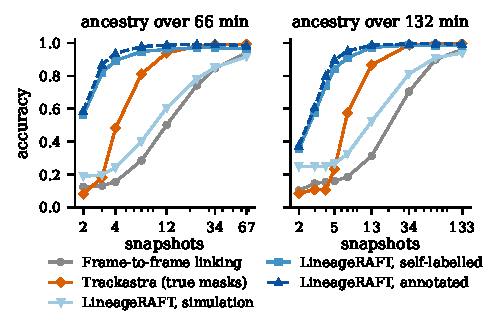
\includegraphics[width=\linewidth]{fig/sparsity.pdf}
\caption{\textbf{How many snapshots does lineage need?} Ancestry over 66 or 132 minutes on OIAM M3/M4 when the colony is imaged $n$ times at equal intervals and per-interval links are composed (32 random windows per gap, weighted by cells). Trackastra: off the shelf, true masks, argmax decoding (chosen on M2). Self-labelled: trained without any annotation.}
\label{fig:sparsity}
\end{figure}

\begin{figure*}[t]
\centering
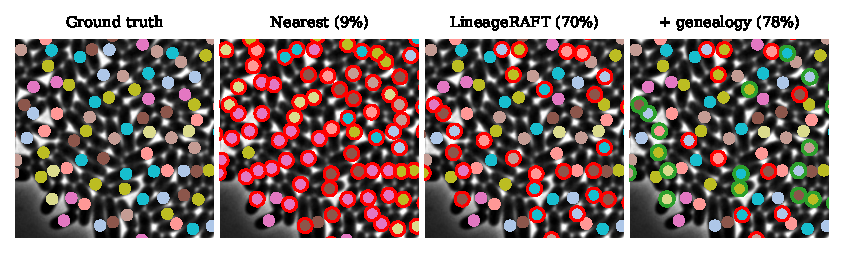
\includegraphics[width=0.74\linewidth]{fig/qualitative.pdf}
\caption{\textbf{A dense OIAM window at a 66-minute gap} (M4, 527 ancestors; crop of the target snapshot). Targets are coloured by their true (left) or predicted ancestor; red rings mark errors, green rings (right) errors of the network that the genealogy decoder corrects; percentages are accuracy over the whole window. Nearest assignment fails because cells moved more than the cell spacing; the genealogy fixes errors where neighbouring families interleave.}
\label{fig:qualitative}
\end{figure*}

\begin{table}[t]
\centering\small
\setlength{\tabcolsep}{3pt}
\begin{adjustbox}{max width=\linewidth}
\begin{tabular}{lccccccc}
\toprule
& \multicolumn{4}{c}{Baselines} & \multicolumn{2}{c}{\ours trained on} & Seq. \\
\cmidrule(lr){2-5}\cmidrule(lr){6-7}
Dataset & Nearest & Radial & Transl. & Other$^*$ & OIAM & \rodsim & wins \\
\midrule
FAST & .596 & .608 & .591 & .618$^{\mathrm{o}}$ & .615 & \textbf{.709} & 7/7 \\
recA & .452 & .470 & .462 & .481$^{\mathrm{o}}$ & .474 & \textbf{.560} & 9/9 \\
rpsM & .425 & .455 & .447 & .464$^{\mathrm{o}}$ & .465 & \textbf{.564} & 9/9 \\
OIAM & .374 & .449 & .345 & .487$^{\mathrm{d}}$ & .498 & \textbf{.520} & 2/2 \\
T98G & .889 & .896 & .898 & \textbf{.941}$^{\mathrm{o}}$ & .814 & .877 & 0/1 \\
LFCT & \textbf{.930} & .868 & .868 & .926$^{\mathrm{o}}$ & .793 & .894 & 0/1 \\
\bottomrule
\end{tabular}
\end{adjustbox}
\caption{\textbf{Zero-shot transfer.} Accuracy averaged over the three gaps of each dataset. Except for the OIAM-trained model on OIAM, no model saw labels from these datasets; the \rodsim model saw no real data at all. $^*$Best per dataset, in hindsight, of OT (o; three settings), CPD (c), Darcy advection (d) and \rodsim forward simulation (f), all fixed on OIAM M0--M2. \ours uses positions only. Last column: sequences on which \rodsim-trained \ours beats the best of all ten baselines (the columns, radial sector and the six behind Other; mean over gaps). \rodsim-trained: mean of three training seeds (per window); OIAM-trained: one seed, three movies, with rotation augmentation.}
\label{tab:external}
\end{table}


\subsection{Learning from simulation alone}
\cref{tab:external} evaluates positions-only \ours on datasets it was never trained on.
The model trained on OIAM M0--M2 barely improves on geometric baselines elsewhere and is worse on the human-cell datasets: it has learned the geometry of one experiment.
The model trained only on \rodsim is the best method on every bacterial dataset, by 3--10 points over the best baseline (three-seed mean), and wins on all 27 bacterial sequences; on FAST, Trackastra with images and true masks reaches 0.63 (pre-registered; Supp.~F).
The transfer is the simulator's: the direct matcher trained on the same simulations does as well (FAST/recA/rpsM/OIAM 0.71/0.57/0.58/0.50 \vs 0.71/0.56/0.56/0.52; pre-registered, Supp.~F). External windows hold 4--6 ancestors, where even in-domain the centre adds 0.01; on crowded OIAM windows the \rodsim-trained centre adds 0.02 (in-domain 0.19); forward simulation with true shapes beats it there (Supp.~Q), and simulating crowded colonies does not help (Supp.~R).
These datasets were seen while the simulator was designed (\cref{sec:sim}), so the clean zero-shot evidence is the blind test of \cref{tab:blind4}.
On the sparse human-cell datasets a baseline is best.


\begin{table}[t]
\centering\small
\setlength{\tabcolsep}{3pt}
\begin{adjustbox}{max width=\linewidth}
\begin{tabular}{llcccccc}
\toprule
 & Lineage & \multicolumn{3}{c}{All windows} & \multicolumn{3}{c}{Dense ($>$200)} \\
\cmidrule(lr){3-5}\cmidrule(lr){6-8}
Training & labels & 33 & 66 & 132 & 33 & 66 & 132 \\
\midrule
\multicolumn{8}{l}{\emph{Positions only, seed 0}} \\
\rodsim only & -- & .665 & .516 & .393 & .340 & .198 & .097 \\
\quad + fine-tune, true lineage & M0--M2 & .719 & .556 & .418 & .458 & .292 & .182 \\
\quad + fine-tune, self-labelled & none & .715 & .564 & .418 & .454 & .292 & .180 \\
\multicolumn{8}{l}{\emph{Full model (shape, Darcy), mean of three seeds}} \\
True lineage & M0--M2 & .957 & .780 & .473 & .907 & .598 & .267 \\
Self-labelled & none & .935 & .733 & .452 & .865 & .533 & .244 \\
\quad without consistency term (post hoc) & none & .940 & .759 & .456 & .877 & .577 & .258 \\
\bottomrule
\end{tabular}
\end{adjustbox}
\caption{\textbf{Self-labelling replaces lineage annotation} (OIAM M3/M4, accuracy, argmax). Self-labelled models are trained on lineage obtained by chaining one-frame links through the \emph{unannotated} M0--M2 time-lapses (\cref{sec:selflabel}); fine-tuning runs 6k steps from the \rodsim model, full models 80k steps from scratch (seed std $\le$0.013).}
\label{tab:selflabel}
\end{table}


\subsection{Self-labelling replaces lineage annotation}
Chaining one-frame links (\cref{sec:selflabel}) through the unannotated OIAM training movies recovers the true ancestor of 0.88--0.98 of cells at horizons of 33 to 240 minutes (Supp.~M).
Without the fission prior's daughter slots, links at divisions are wrong 30\% of the time instead of 4\% (pseudo-lineage at 132 minutes: 0.57 \vs 0.92).
\cref{tab:selflabel} trains on this pseudo-lineage instead of the annotation.
Fine-tuning the \rodsim model on it gains as much as on true lineage, and the full model trained from scratch on it comes within 0.02--0.05 of the annotated one over all windows (three seeds; \cref{tab:selflabel}); self-labelling costs the direct matcher only 0.01, yet self-labelled \ours beats the direct matcher trained on true lineage at 33/66 minutes (+0.08/+0.05; pre-registered, Supp.~M).
Self-labelling the genealogy network too (AP within 0.02; Supp.~K) removes annotation from every step: decoded ensembles reach 0.963/0.822/0.487 (fixed beforehand) \vs 0.977/0.863/0.517 (\cref{tab:oiam}).

\begin{table}[t]
\centering\small
\setlength{\tabcolsep}{4pt}
\begin{adjustbox}{max width=\linewidth}
\begin{tabular}{lcccccccc}
\toprule
Subset & $n$ & Best geom. & Best other & \rodsim & + Hung. & + boot. & \multicolumn{2}{c}{wins} \\
\cmidrule(lr){8-9}
 & & & & & & & \rodsim & boot. \\
\midrule
trpL & 10 & .574 & .591 & .674 & .598 & \textbf{.711} & 10/10 & 10/10 \\
metA & 9 & .497 & .517 & .636 & .542 & \textbf{.668} & 9/9 & 9/9 \\
pheA & 9 & .520 & .545 & .667 & .588 & \textbf{.714} & 9/9 & 9/9 \\
\bottomrule
\end{tabular}
\end{adjustbox}
\caption{\textbf{Pre-registered blind test} on three \emph{E.~coli} subsets of~\cite{vanvliet2018spatially} in minimal medium, never downloaded before the protocol was fixed (accuracy: mean over colonies of the mean over 30/60/120-minute gaps; run once). Best geom.: of nearest, translation, radial expansion and radial sector; best other: of exact and unbalanced OT (tuned on OIAM) and, added afterwards, radial-aligned OT, CPD, Darcy and forward simulation. Hung./boot.: \rodsim model fine-tuned on Hungarian-chained or bootstrapped pseudo-lineage of the other fold. Wins: colonies where \rodsim beats all ten baselines (also the six pre-registered), and where bootstrapping beats \rodsim.}
\label{tab:blind4}
\end{table}


\subsection{Pre-registered blind tests}
On unseen data we fixed each protocol, hypotheses included, before running it, and report every outcome (ledger: Supp.~O).
The first two failed instructively: on TrackRefiner~\cite{ahmadi2025trackrefiner} and TrackMate~\cite{anselmet2026trackmate} the \rodsim model won only on the 2 of 11 sequences showing a single colony (the others hold many microcolonies or are steady-state chambers), and on static \emph{B.~subtilis} spores~\cite{kunzmann2026bsub} nearest assignment is best.
Per-colony processing (post hoc) and self-labelling within each source (fixed beforehand) recover much of this, budding yeast~\cite{zelic2026lyn} included (Supp.~N).

A last test, with these procedures fixed, used three unused subsets of~\cite{vanvliet2018spatially}: 28 \emph{E.~coli} microcolonies in minimal medium from the lab and pipeline of recA/rpsM (\cref{tab:blind4}).
All four hypotheses hold on all three subsets: zero-shot, the \rodsim model beats every baseline on all 28 colonies, by 0.10 on average (95\% CI 0.09--0.11), and bootstrapped self-labelling from the other fold raises it further on all 28, whereas positions-only Hungarian self-labels lower it.



\begin{table}[t]
\centering\small
\setlength{\tabcolsep}{4pt}
\begin{adjustbox}{max width=\linewidth}
\begin{tabular}{llccc}
\toprule
Training data & Input & 33 & 66 & 132 \\
\midrule
& Base rate & .057 & .093 & .185 \\
OIAM M0--M2 & Geometry & .764 & .686 & .540 \\
OIAM M0--M2 & Image + geometry & .970 & .911 & .701 \\
\rodsim & Geometry & .088 & .119 & .201 \\
\rodsim & Image + geometry & .116 & .226 & .360 \\
\rodsim + division modes & Geometry & .490 & .491 & .460 \\
\rodsim + division modes & Image + geometry & .534 & .502 & .465 \\
\bottomrule
\end{tabular}
\end{adjustbox}
\caption{\textbf{Genealogy is visible in one snapshot.} Average precision for ``same ancestor $H$ minutes ago'' over 8-nearest-neighbour pairs in single OIAM M3/M4 frames. \rodsim rows use no real label; division-modes rows also render lineage (inherited intensity, septum constriction; alone: AP .110/.166/.219).}
\label{tab:genealogy}
\end{table}


\subsection{Genealogy from a single snapshot}
A single image carries much of the family structure that geometry lacks (\cref{tab:genealogy}).
At 33 minutes, where the positive pairs are mostly sisters from the last division, the image model reaches 0.97 AP against 0.76 for geometry and a 6\% base rate; even at 132 minutes it reaches 0.70 against 0.54.
Trained on \rodsim, it transfers only once division modes are randomised (V-snapping~\cite{messelink2021single}; added after inspecting OIAM M3), and then mostly through geometry (AP 0.53/0.50/0.47; 0.49/0.49/0.46 without the image).
In the Potts decoder ($\beta{=}2$, fixed), the image affinities improve every base model at every gap; the full model gains 0.034 at 66 minutes, the three-seed ensemble 0.057 (single models are overconfident; Supp.~I).
The decoder also lifts fine-tuned Trackastra at 33/66 minutes, yet decoded \ours stays ahead (pre-registered; Supp.~I). Non-local partitioners, a fission prior on family size and ancestors competing inside refinement leave 132-minute accuracy unchanged (the last helps dense windows; Supp.~I, R).


\subsection{Robustness to detection errors}
With 10\% of cells missed, merged or hallucinated, \ours is still 90--91\% correct at 33 minutes (nearest: 50\%).
With untuned Cellpose-SAM~\cite{pachitariu2025cellposesam} masks, \ours reaches 0.92/0.73/0.44; Omnipose~\cite{cutler2022omnipose} adds debris to sparse frames (0.74/0.50/0.29; Supp.~L).

\subsection{Limitations}
End-to-end results cover two segmenters on one dataset; synthetic detection errors ignore image content.
Trained from scratch on two annotated movies, \ours trails fine-tuned Trackastra (0.72 \vs 0.89 at 33 minutes; Supp.~F). OIAM's five movies are one experiment (the only public crowded lineage data we found), and the zero-shot advantage vanishes on fields of many tiny colonies or steady-state chambers.
Self-labelling needs a dense time-lapse per condition and inherits fast-motion linking errors (TrackRefiner).

\section{Conclusion}
\label{sec:conclusion}
Two snapshots of a growing population an hour apart hold more lineage than trackers extract, even fine-tuned at the gap.
Registering families recovers most of it at short and medium gaps, without annotation: simulation transfers across colonies, binary fission turns time-lapses into near-annotation labels, and one image reveals close relatives.
Long gaps need centres and partitions inferred jointly; until then, one extra snapshot halfway beats any model change we tried.

{
    \small
    \bibliographystyle{ieeenat_fullname}
    \bibliography{main}
}
\end{document}
